% include the figures path relative to the master file
\graphicspath{ {./content/method/figures/} }
\section{Background}\label{sec:review}
This section reviews works straightly addressing the problem of classifying \gls{oct} volumes as normal or abnormal, regardless of the targeted pathology.
The methods are categorized in terms of their learning strategy, namely supervised or semi-supervised learning.


\subsection{Supervised methods}
% Common framework
% \added[id=mojh]{
%   All the previously mentioned methods follow a similar pipeline or framework, which consists of different steps.
%   We categorized these steps as pre-processing, feature extraction, mapping, feature representation and finally classification, as it is shown in Fig.\,\ref{fig:ML-scheme}.

%   Pre-processing of \gls{oct} volumes, as noted in Sect.~\ref{sec:review}, consists of denoising, flattening the retinal curvature, aligning the B-scans through the whole volume and finally cropping or resizing the volumes.
%   Feature extraction refers to extraction of different textural and shape information from the B-scan or the volumes.
%   Mapping step is used to determine a discrete set of elements (structures) representing a sample (i.e.B-scan/volume).
%   In this step either one structure is used per sample namely global-mapping or the features are extracted with reference to a set of structures, i.e.dense or sparse patches through the sample, local-mapping.

%   In feature representation step, the representation of the final descriptor prior to classification is decided.
%   The extracted features using different mapping techniques can be represented in lower dimensions (using \gls{pca} for instance), as a concatenated of descriptor, histogram of words (using \gls{bow}) or sparse representation (sparse coding).
% }

Supervised learning is based on a fully annotated and labeled training set.
In this approach, the labeled training data are used to train the classifier function later used for prediction.
% Semi-supervised classification takes advantage of both unlabeled and labeled data.
% This techniques are particularly useful when there is lack of annotated data moreover it has shown that use of small amount of labeled data in conjunction of unlabeled data can increase the learning accuracy.
%
Figure~\ref{fig:ML-scheme} illustrates a prevalent framework for supervised learning.
Each \gls{sdoct} volume undergoes:
(i)~\emph{pre-processing} to reduce noise and other acquisition deficiencies which alter the images;
(ii)~\emph{feature detection} to quantify visual cues like appearance, texture, shape;
(iii)~\emph{mapping} in which a sample is either considered as whole (i.e., global) or partitioned into a set of sub-elements (i.e., local dense/sparse patches, pyramid, etc.);
(iv)~\emph{feature representation} to associate a descriptor (e.g., concatenation, statistics, histogram, \gls{pca}, \gls{bow}, etc.) for each element from the \emph{mapping-stage}.
This descriptor packages the visual cues associated to the sample;
(v)~\emph{classification} to determine which class has to be affected to the given sample.

% The details implementation of the following methods and their integration to our common framework is described in Sect.~\textit{experiments}.

\begin{figure*}
  \centering{
  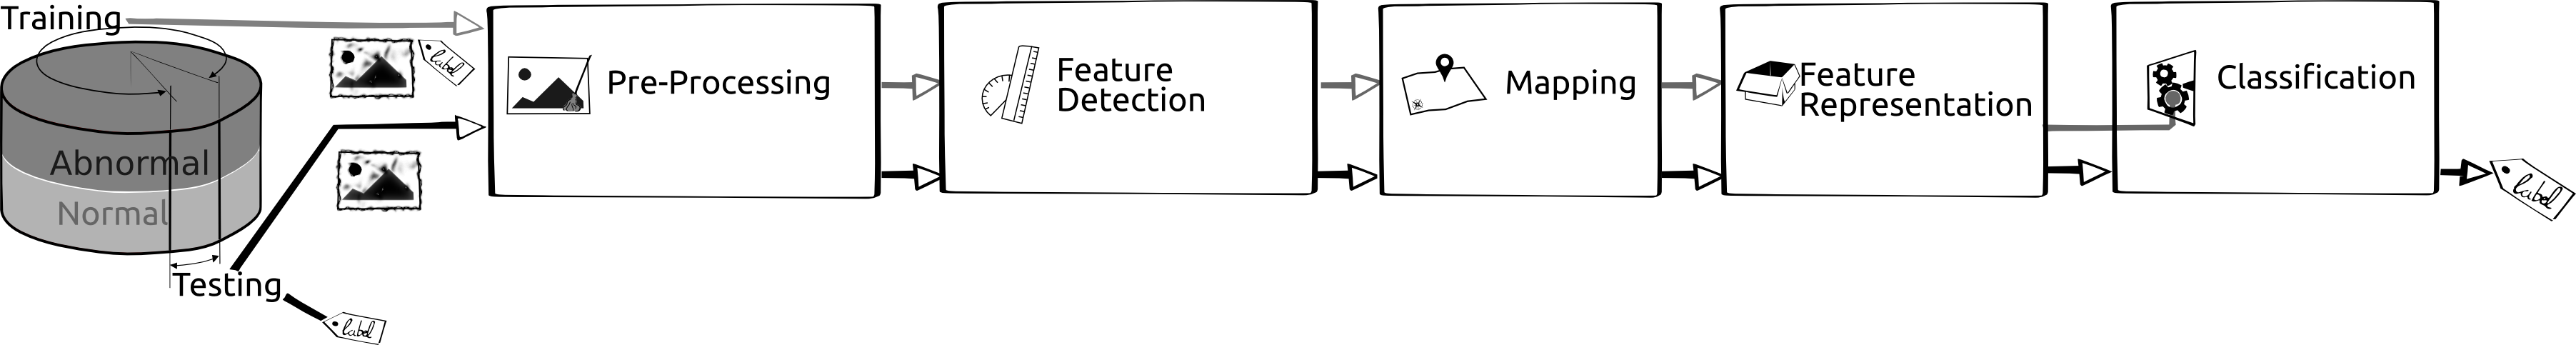
\includegraphics[width=1\linewidth]{ml-2}}
  \caption{Common framework}
  \label{fig:ML-scheme}
\end{figure*}

%%% Venhuizen2015
%
% Brief method description (or goal)
Venhuizen~\textit{et~al.} propose a classification method to distinguish between \gls{amd} and normal \gls{sdoct} volumes using \gls{bow} models~\cite{Venhuizen2015}.
%
% Method description
A set of keypoints are detected and selected at each individual B-scan, by keeping the salient points included in the top $3 \%$ of the vertical gradient values.
Around each of these keypoints, a \SI[product-units=repeat]{9x9}{\px} texton is extracted, generating a feature vector of $81$ dimensions, later reduce to $9$ using \gls{pca}.
All extracted feature vectors are used to create a codebook using \textit{k}-means clustering.
Then, each \gls{oct} volume descriptor is represented as a histogram that captures the codebook occurrences and are later used to train a \gls{rf} composed of $100$ trees.
%
% Reported results
The method is tested using a publicly available dataset of $384$ \gls{oct} volumes~\cite{farsiu2014quantitative}, achieving an \gls{auc} of $0.984$.

%%% Srinivasan2014
%
% Brief method description (or goal)
Srinivasan~\textit{et~al.} propose a classification method to distinguish \gls{dme}, \gls{amd}, and normal \gls{sdoct} volumes~\cite{Srinivasan2014}.
%
% Method description
Each \gls{oct} slice is pre-processed using \gls{bm3d} to reduce the speckle noise and is flattened to reduce the inter-patient retinal curvature variations.
A multi-resolution pyramid is generated for each pre-processed slice and a \gls{hog} feature is computed for each layer.
These features are classified using a linear \gls{svm}.
Note that each individual B-scan is classified into one of the three categories, namely \gls{dme}, \gls{amd}, and normal, and a volume is affected to the class by taking the majority vote of all B-scans.
%
% Reported results
This method is also tested using a publicly available dataset, composed of $45$ patients equally subdivided into the three targeted classes.
Correct classification rates of $100 \%$, $100 \%$ and $86.67 \%$ are obtained for normal, \gls{dme}, and \gls{amd} patients, respectively.
% The images that have been used in their paper, are publicly available but are already preprocessed (i.e., denoised), have different sizes for the \gls{oct} volumes, do not offer a huge variability in term of \gls{dme} lesions, and some of them, without specifying which, have been excluded for the training phase; all these reasons prevent us from using this dataset to benchmark our work.

Alsaih~\emph{et~al.} extended the previous work~\cite{Alsaih2016apr-repoICPR}, incorporating \gls{lbp} to \gls{hog} and reducing the number of dimension using \gls{pca}, similarly to Venhuizen~\textit{et~al.}.

Lema\^itre~\emph{et~al.} propose a method based on \gls{lbp} features to describe the texture of \gls{oct} images and dictionary learning using the \gls{bow} models~\cite{Lemaintre2015miccaiOCT}.
%Note that using \gls{bow} and dictionary learning contrary to \cite{Srinivasan2014} the classification is performed per volume, rather than B-scan.
In this method, the \gls{oct} images are first pre-processed using \gls{nlm} filtering, to reduce the speckle noise.
%The data is pre-processed using \gls{nlm} filtering.
Then, the volumes are mapped into a discrete set of structures: (i) local corresponding to patches, or (ii) global corresponding to volume slices or the whole volume.
According to the chosen mapping, \gls{lbp} or \gls{lbptop} texture features are extracted and represent each volume through histogram, \gls{pca}, or \gls{bow} representation.
The final feature descriptors are classified using \gls{rf} classifier.
This methodology is tested against Venhuizen~\textit{et~al.}~\cite{Venhuizen2015} using public and non-public datasets showing an improvement within the results by achieving a \gls{se} of $87.5 \%$ and a \gls{sp} of $75 \%$.

%
% description
Liu~\textit{et~al.} propose a methodology aiming at classifying B-scan rather than volume.
The classification goal is to distinguish between macular pathology and normal \gls{oct} B-scan images using \gls{lbp} and gradient information as attributes~\cite{Liu2011}.
%
% Method description
Each \gls{oct} slice are flattened before to create a $3$-level mutlti-scale spatial pyramid.
From each layer of this pyramid, edges are extracted and \gls{lbp} descriptors are computed for the flattened slice and the edge map.
%is created and edge and \gls{lbp} histograms are extracted in each block at every level of the pyramid.
All the obtained histograms are concatenated into a global descriptor whose dimensions are reduced using \gls{pca}.
Finally, a \gls{svm} with an \gls{rbf} kernel is used as classifier.
%
% results report
The method achieved good detection performance of \gls{oct} scan containing different pathologies with an \gls{auc} of $0.93$ using a dataset of $326$ \gls{oct} scans.

%Albarrak paper
% description
Albarrak~\textit{et~al.}~\cite{albarrak2013age} propose another volumetric classification framework for differentiating \gls{amd} and normal volumes.
%
% Method description
The author propose to flatten the \gls{voi} from each \gls{oct} volume as a pre-processing step and extract \gls{lbptop} and \gls{hog}+\gls{lbptop} features from individual sub-volumes within each \gls{voi}.
The extracted features were concatenated into a single feature vector per \gls{oct} volume and presented in lower dimensions using \gls{pca}.
Finally a Bayesian network classifier was used for classifying the volumes.
%
%results
Testing their proposed method and comparing with \cite{Liu2011} using 140 \gls{oct} volumes, they achieved the highest \gls{se} and \gls{sp} of 92.4\% and 90.5\%, respectively.

% Anantrairichai paper
% description
Anantrasirichai~\textit{et~al.}~\cite{anantrasirichai2013svm} propose to detect glaucoma in \gls{oct} images based on a variety of texture measures.
%
%Method description
The images are described in terms of \gls{lbp}, \gls{glcm}, wavelet, granulometry, run length measures, and intensity level distributions in combination with retinal layer thickness without any pre-processing.
Using \gls{pca} and linear and kernel-\gls{svm} classifier, the authors compared the performance of individual features and their combinations.
%
% results
Testing with rather a small dataset of 24 \gls{oct} voluems, their proposed method achieved an \gls{acc} of 81.95\% while using layer thickness information.


\subsection{Semi-supervised methods}
An example of semi-supervised approach for \gls{sdoct} classification is recently proposed by Sankar~\textit{et~al.}~\cite{sankar2016classification}.
The proposed method is based on appearance modeling of normal \gls{oct} images using \gls{gmm} and anomaly detection.
The abnormal B-scans are detected as outliers to the fitted \gls{gmm} and volume classification is performed based on the number of detected outliers in the volume.

%The proposed method is based on modeling the appearance of the normal \gls{oct} images using a \gls{gmm} and detecting abnormal \gls{oct} images as outliers.
%Use an anomaly detection approach to identify abnormal B-scan as outliers to the \gls{gmm} and finally detect unhealthy \gls{oct} volumes based on the number of abnormal B-scan.
This approach differs from supervised approaches since the B-scan detection method does not require a labeled training set of B-scans.
This method starts by pre-processing the B-scans using resizing, flattening and denoising (\gls{nlm} filter).
The features are extracted by taking the intensity information of each B-scan and applying \gls{pca} to reduce their dimension.
The feature space is then modeled using \gls{gmm}.
In the testing stage, for the new B-scan, the features are extracted in a similar way and they are classified as normal or abnormal based on their Mahalanobis distance to the \gls{gmm}.
Finally the volume classification is performed considering the umber of outliers (abnormal) B-scans per volume.

% \begin{landscape}
\begin{table}
\caption{Summary of the state-of-the-art methods.}
\resizebox{1.05\linewidth}{!}{
\scriptsize{
\begin{tabular}{l ccc c cccc	c c c c	c c}
\toprule
Ref & \multicolumn{3}{c}{Diseases} & Data  & \multicolumn{4}{c}{Pre-processing} & Features & Representation & Classifier & Evaluation & Results\\
    &  &  &  & size &  &  &  &  &  &  &  & & &\\
   \cmidrule(l){2-4}\cmidrule(l){6-9} 
    & \gls{amd} & \gls{dme} & Normal  &           & De-noise & Flatten & Aligning & Cropping &   & &   &  &   \\
\midrule
& & & & & & & & & & & & & &  \\
%Srinivansan\,\textit{et al.}~
\cite{Srinivasan2014} & $\checkmark$ & $\checkmark$ & $\checkmark$ &  45 & $\checkmark$ & $\checkmark$ &  & $\checkmark$ & \gls{hog} &  & linear-\gls{svm} & \gls{acc} & 86.7\%,100\%,100\%  \\
& & & & & & & & & & & & &    \\
%Venhuizen\,\textit{et al.}~
\cite{Venhuizen2015} & $\checkmark$ &  & $\checkmark$ & 384 &  & & & &  Texton  &\gls{bow}, \gls{pca}  & \gls{rf} & \gls{auc} & 0.984 \\ 
& & & & & & & & & & & & &   & \\
%Liu\,\textit{et al.}~
\cite{Liu2011} & $\checkmark$ & $\checkmark$ & $\checkmark$  & 326 &  & $\checkmark$ & $\checkmark$ &  &  Edge, \gls{lbp} & \gls{pca}& \gls{svm}-\gls{rbf} &\gls{auc} & 0.93 \\
& & & & & & & & & & & & & \\
%Lema\^itre\,\textit{et al.}~
\cite{Lemaintre2015miccaiOCT} &  & $\checkmark$ & $\checkmark$ & 62  & $\checkmark$ &  &  &  & \gls{lbp}-\gls{lbptop} & \gls{pca}, \gls{bow}, histogram&  \gls{rf} & \gls{se},\gls{sp} & 87.5\%, 75\%  \\
& & & & & & & & & & & & &  \\
\bottomrule
\end{tabular}}}
\label{tab:survey-tab}
\end{table}

\graphicspath{ {./content/method/figures/ml_schema/} }
\begin{figure}
  \centering{
    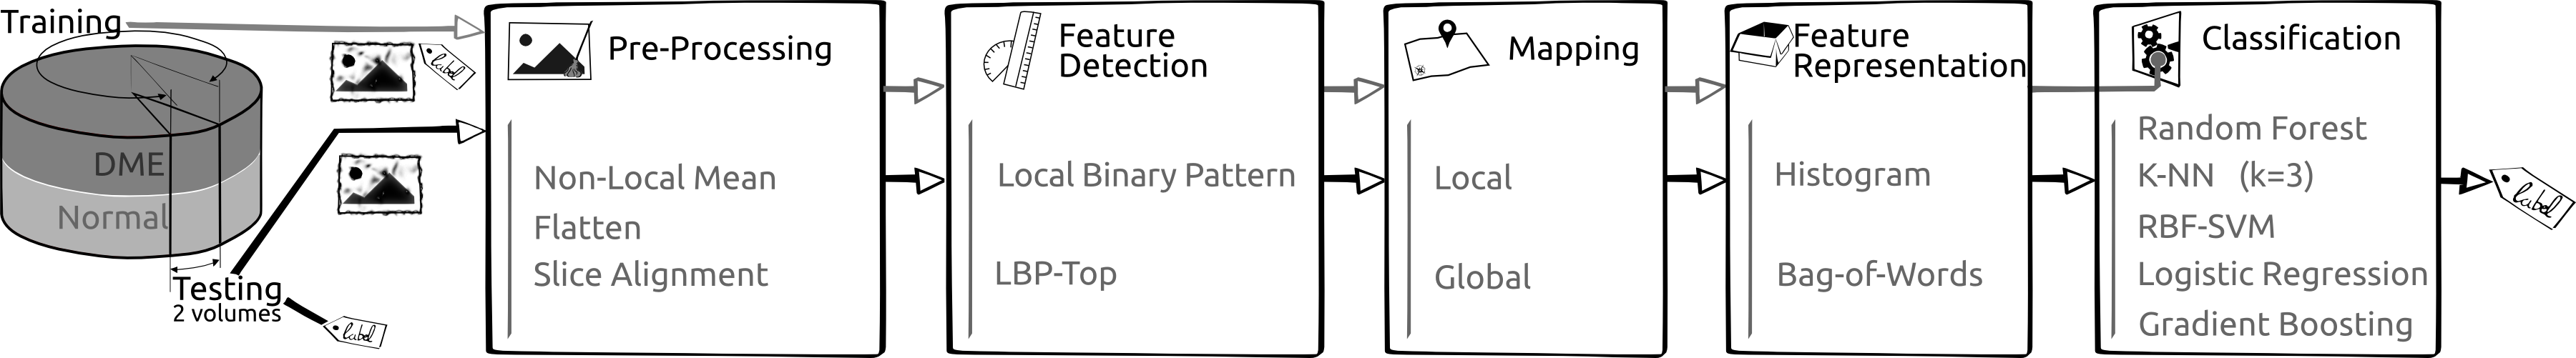
\includegraphics[width=1\linewidth]{ml}}
    \caption{Our proposed classification pipeline.}
  \label{fig:ML-scheme}
\end{figure}



\end{landscape}

